\section{GPT辅助开发与代码编写}\label{sec:gpt-code}


在这个数字化时代,编程已经成为连接人类智慧与机器世界的桥梁。从智能手机到人工智能,每一行代码都在构建着我们未来的数字文明。但编程并非易事,它需要深奥的知识、严谨的逻辑和丰富的经验。

而GPT(生成式预训练变换模型)的出现,正在改变这一现状。这项革命性的技术不仅能够理解人类的语言,更能理解和生成高质量的代码。这不仅是技术创新的进步,更是人类智慧与机器智能融合的新起点。

本节将带读者进入这个激动人心的技术领域,探索GPT如何成为每一位开发者的强大助力。无论您是编程新手还是经验丰富的开发者,都将在这里发现新的可能性,开启代码创作的新纪元。

\subsection{使用GPT进行代码开发}\label{sec:gpt-dev}

在传统的软件开发过程中,开发者面临着一系列复杂且相互关联的任务。首先,需求理解是软件开发的起点,开发者需要将业务需求准确地转化为技术实现的方案。这一过程不仅要求开发者具备对业务的深刻洞察力,还需要他们能够将非技术性的需求转化为清晰、可操作的技术目标。随后,系统设计阶段要求开发者规划整个系统的架构和模块划分,这需要他们在宏观层面把握系统的整体结构,同时确保各个模块之间的协同性和可扩展性。编码实现阶段则是将设计转化为实际代码的过程,开发者需要编写高质量的代码,以确保软件的性能和可靠性。最后,测试与维护阶段是软件开发的收尾环节,开发者需要确保代码的稳定性和可维护性,以便在软件的生命周期中持续优化和更新。这些环节不仅耗时耗力,还要求开发者具备跨领域的知识,涉及业务理解、架构设计、编程技能以及质量保证等多个方面。

然而,随着人工智能技术的飞速发展,特别是像 GPT 这样的大型语言模型的出现,为解决这些传统软件开发中的难题提供了新的思路和方法。这些模型能够通过自然语言理解与生成的能力,辅助开发者在需求理解阶段更准确地把握业务需求,甚至自动生成初步的设计方案和代码框架。在测试与维护阶段,它们也能提供自动化测试脚本生成和代码优化建议等支持,从而显著提高软件开发的效率和质量。

GPT 作为一种先进的人工智能语言模型,正在通过多种方式深刻地改变传统的软件开发模式。首先,它能够实现自动化生成文档的功能,这使得开发者可以高效地根据现有代码自动生成 API 说明和用户手册等文档资料。这种自动化文档生成不仅节省了开发者在文档编写上的大量时间,还确保了文档与代码的一致性和准确性,从而提高了开发效率和软件交付的质量。
其次,GPT 在智能代码审查方面发挥着重要作用。它能够对代码进行深度分析,提供有价值的改进意见,并帮助开发者发现潜在的问题。这种智能审查功能类似于一个虚拟的代码导师,能够在开发过程中及时指出代码中的不足之处,从而帮助开发者优化代码质量,减少错误和漏洞。
此外,GPT 还支持快速原型开发。开发者只需提供需求描述,GPT 就能够快速生成初始的代码框架。这种能力极大地缩短了从需求分析到代码实现的时间,使得开发者能够更快速地验证想法并进行迭代开发。快速原型开发不仅提高了开发效率,还降低了项目初期的风险,使团队能够更快地响应市场变化。
最后,GPT 提供了跨语言支持功能,能够在不同编程语言之间进行代码转换和适配。这一功能对于多语言开发环境尤为重要,它使得开发者能够在不同语言之间无缝切换,减少了因语言差异带来的开发障碍。跨语言支持不仅提高了开发的灵活性,还促进了不同技术栈之间的协作和整合。

因此,选择 GPT 是因为它能够显著提高开发效率,减少重复性工作并加速流程;通过智能检查提升代码质量,增强稳定性和可维护性;有效连接业务需求与技术实现,弥合二者之间的鸿沟;同时为创新提供可能,探索传统方法难以触及的解决方案,从而推动软件开发向更高层次的效率、质量和创新能力迈进。这些功能不仅提高了开发效率,还提升了软件的整体质量,为软件开发领域带来了新的可能性和机遇。

下面通过实际的例子来展示GPT在开发中的应用。以网站开发为例,先介绍生成API文档,由用户输入代码片段,由GPT输出详细的接口说明:

\begin{promptbox}
\small{
\begin{lstlisting}[language=Python]
    // 用户输入一段REST API的代码
    GET /users
    Response:
    \{
        "users": [
            {"id": 1, "name": "Alice"},
            {"id": 2, "name": "Bob"}
        ]
    \}
\end{lstlisting}}
\end{promptbox}

\begin{gptbox}
\small{
\begin{lstlisting}[language=Python]
    // GPT生成的API文档
    ### 用户管理接口
    
    #### 获取用户列表
    ```http
    GET /api/users
    
    
    #### 响应格式
    \{
        "users": [
            {"id": number, "name": string}
        ]
    \}

    #### 错误码
    401: 未认证
    500: 内部错误
    ...
\end{lstlisting}
}
\end{gptbox}


除此之外,对于已经编写好的代码,用户还可以使用GPT对代码审查与优化,用户原始代码输入如下:

\begin{promptbox}
\small{\begin{lstlisting}[language=Python]
    # 用户输入的原始代码
    def calculate_average(numbers):
        sum = 0
        for number in numbers:
            sum += number
        average = sum / len(numbers)
        return average
\end{lstlisting}}
\end{promptbox}

\begin{gptbox}
\small{
\begin{lstlisting}[language=Python]
    # GPT建议的优化版本
    def calculate_average(numbers):
        """计算数字列表的平均值"""
        if not numbers:
            return 0.0
        return sum(numbers) / len(numbers)
\end{lstlisting}
}
\end{gptbox}

快速原型开发是GPT在代码开发的重要应用,体现了GPT独立完成开发项目的能力。从用户需开始,描述如下:

\prompt{需要一个在线投票系统,用户可以创建投票、查看结果统计。}


\begin{gptbox}
\small{
\begin{lstlisting}[language=Python]
    # models.py
    class Poll(models.Model):
        title = models.CharField(max_length=200)
        description = models.TextField()
        created_at = models.DateTimeField(auto_now_add=True)
        votes = models.ManyToManyField(User, through='Vote')
    
    class Vote(models.Model):
        user = models.ForeignKey(User, on_delete=models.CASCADE)
        poll = models.ForeignKey(Poll, on_delete=models.CASCADE)
        choice = models.CharField(max_length=200)
    
    # views.py
    @login_required
    def create_poll(request):
        if request.method == 'POST':
            form = PollForm(request.POST)
            if form.is_valid():
                poll = form.save(commit=False)
                poll.created_by = request.user
                poll.save()
                return redirect('poll_list')
        else:
            form = PollForm()
        return render(request, 'create_poll.html', {'form': form})
\end{lstlisting}
}
\end{gptbox}


\subsection{使用GPT进行代码编写}

在日常编程实践中,开发者常常遭遇诸多棘手难题,这些问题不仅影响开发效率,还可能引发潜在的软件质量问题。首先,语法错误是编程中常见的问题,包括拼写错误、括号不匹配等,这些问题虽小,却能导致程序无法正常编译或运行。其次,逻辑问题往往更具挑战性,例如算法的实现、复杂的条件判断以及程序流程的控制,这些问题需要开发者具备深入的逻辑思维能力和丰富的编程经验。此外,代码风格的统一性也是一个不容忽视的问题,保持代码的一致性和可读性对于团队协作和后续维护至关重要,然而在实际开发中,由于不同开发者编程习惯的差异,代码风格往往难以统一。最后,知识获取也是开发者面临的一大挑战,快速准确地查找 API、框架的使用方法以及相关技术文档,对于高效开发至关重要,但在海量信息中筛选出准确、有用的内容并非易事。

在这种背景下,GPT 的出现为解决上述问题提供了创新性的思路和方法。凭借其强大的语义理解和生成能力,GPT 能够在多个层面为开发者提供支持。它不仅可以帮助开发者快速识别和纠正语法错误,还能通过逻辑分析和代码优化建议,协助解决复杂的逻辑问题。此外,GPT 还能够提供代码风格指南和格式化建议,帮助开发者保持代码的一致性和可读性。更重要的是,GPT 能够快速响应开发者关于 API 和框架使用方法的查询,提供准确的技术信息,从而显著提升开发效率并降低知识获取的门槛。

同时,在软件开发领域,编码效率的提升是开发者不懈追求的目标。GPT 作为一种先进的人工智能工具,为这一目标的实现提供了强有力的支持。首先,GPT 的智能代码补全功能能够根据上下文环境精准预测下一步代码,极大地减少了开发者手动输入代码的时间,同时降低了因拼写错误或语法不规范而导致的编译问题。其次,GPT 能够识别代码中的错误,并提供针对性的修正建议,这不仅帮助开发者快速定位问题,还提升了代码的可靠性和稳定性。此外,GPT 还具备代码风格调整的能力,能够统一代码格式并优化变量命名,从而增强代码的可读性和一致性。最后,GPT 可以即时获取 API 说明和使用示例,为开发者提供技术文档查找的便捷途径,显著减少了在海量信息中搜索所需知识的时间成本。

选择 GPT 作为开发辅助工具,不仅因其能够提供即时帮助,随时为开发者提供编程指导和建议,还在于其能够显著提升代码质量。通过智能纠错功能,GPT 有效减少了潜在的错误,增强了代码的可靠性,从而为软件的稳定性和可维护性奠定了坚实基础。此外,GPT 的使用大幅节省了开发者查找资料的时间成本,使他们能够将更多精力集中在核心逻辑的实现上。更为重要的是,GPT 能够启发开发者探索新的解决方案和实现方式,为软件开发带来创新思路。这些优势共同构成了 GPT 在软件开发领域广泛应用的重要原因,使其成为开发者提升编码效率和质量的得力助手。

为了充分发挥GPT的代码编写能力,下面演示根据自然语言生成代码的过程。

\prompt{我需要一个函数,可以计算两个数的和,并返回结果。}

\begin{gptbox}
\footnotesize{使用如下代码可以实现上述功能:}
\small{
\begin{lstlisting}[language=Python]
    def add_numbers(a, b):
        """Calculate the sum of two numbers."""
        return a + b
\end{lstlisting}
}
\end{gptbox}

\prompt{print("Hello World!)这行代码有没有错误?}

\begin{gptbox}
\footnotesize{检测到缺少引号,应修正为:}
\small{
\begin{lstlisting}[language=Python]
    print("Hello World!")
\end{lstlisting}
}
\end{gptbox}


\begin{promptbox}
\footnotesize{下面的代码效率如何,能不能改进?}
\small{
\begin{lstlisting}[language=Python]
    total = 0
    for num in numbers:
        total += num
    average = total / len(numbers)
\end{lstlisting}}
\end{promptbox}

\begin{gptbox}
\footnotesize{可以使用更简洁的方式:}
\small{
\begin{lstlisting}[language=Python]
    average = sum(numbers) / len(numbers) if numbers else 0
\end{lstlisting}
}
\end{gptbox}



\begin{promptbox}
\footnotesize{帮我统一命名规范}
\small{
\begin{lstlisting}[language=Python]
    function getUserName(id) {
        return users[id].name;
    }
    
    function GetUserEmail(id) {
        return users[id].email;
    }
\end{lstlisting}}
\end{promptbox}

\begin{gptbox}
\footnotesize{以下是统一后的结果}
\small{
\begin{lstlisting}[language=Python]
    function getUserInfo(id, field) {
        return users[id][field];
    }
\end{lstlisting}
}
\end{gptbox}

\subsection{动手试试:明文加密}

正所谓古人云:``学而不思则罔,思而不学则殆''。在前面的介绍中,已经有了实例演示的例子。那么现在我们再尝试动手使用GPT写几个小例子吧\textasciitilde{}。

\paragraph{摩尔斯电码(Morse code)}也被称作摩斯密码,是一种时通时断的信号代码,通过不同的排列顺序来表达不同的英文字母、数字和标点符号。它发明于1837年,是一种早期的数字化通信形式。不同于现代化的数字通讯,摩尔斯电码只使用零和一两种状态的二进制代码,它的代码包括五种:短促的点信号``・'',保持一定时间的长信号``---'',表示点和划之间的停顿、每个词之间中等的停顿,以及句子之间长的停顿。
读者往往会在在众多影视作品中可以看到摩尔斯电码,那么现在我们就让GPT来完成一个这样的简单例子。

\prompt{现在我想编写一个将自然语言转化为摩斯密码的代码,使用Python代码实现,就以''I LIKE U``这个句子为例实现一下。}

\begin{gptbox}
\footnotesize{为了将自然语言句子转换为摩斯密码,我们可以按照以下步骤实现:

\begin{enumerate}
  \def\labelenumi{\arabic{enumi}.}
  \item
        \textbf{创建摩斯密码字典}:包含所有英文字母及其对应的摩斯码。
  \item
        \textbf{处理输入字符串}:将其转为大写,并去除非字母字符,分割成单词列表。
  \item
        \textbf{转换每个单词}:将每个字母转换为摩斯码,并用单个空格分隔。
  \item
        \textbf{合并单词间的摩斯码}:使用三个空格分隔不同单词。
\end{enumerate}
以下是完整的Python代码:
}
\small{
以下是统一后的结果:
\begin{lstlisting}[language=Python]
    # 创建摩斯密码字典
    mos_codes = {
        'A': '.-', 'B': '-...', 'C': '-.-.', 'D': '-..', 'E': '.', 
        'F': '..-.', 'G': '--.', 'H': '....', 'I': '..', 'J': '.---', 
        'K': '-.-', 'L': '.-..', 'M': '--', 'N': '-.', 'O': '---', 
        'P': '.--.', 'Q': '--.-', 'R': '.-.', 'S': '...', 'T': '-', 
        'U': '..-', 'V': '...-', 'W': '.--', 'X': '-..-', 'Y': '-.--', 
        'Z': '--..'
    }
    
    # 获取输入并处理
    input_str = input("请输入要转换的句子:").upper()
    cleaned = ''.join([c if c in mos_codes or c == ' ' else '' for c in input_str])
    words = cleaned.split()
    
    # 转换为摩斯码
    morse_words = []
    for word in words:
        morse_word = [mos_codes[char] for char in word]
        morse_words.append(' '.join(morse_word))
    
    # 合并单词之间的空格
    final_morse = '   '.join(morse_words)
    print(final_morse)
\end{lstlisting}
}
\end{gptbox}

这段代码能够将输入句子转换为对应的摩斯密码,每个字母用单个空格分隔,单词之间用三个空格分隔。
通过本地运行代码并输出字符串``I LIKE U'',读者将得到上面实例的最终输出结果``.. .-.. .. -.- . ..-'',如\reffig{fig:morse}所示。

\fig[h]{
    
\includegraphics[width=0.7\textwidth]{assets/figures/image-20250210171257118.png} %插入图片,[]中设置图片大小,{}中是图片文件名
    \caption{摩斯密码输出} %最终文档中希望显示的图片标题
    \label{fig:morse} %用于文内引用的标签
}

现在读者可以用摩斯密码对你想说的文字进行加密了,读者还可以尝试继续让GPT改进,让这个简单代码不断完善并且可以处理中文相关的信息。

\paragraph{恺撒密码(Caesar cipher)},或称\textbf{恺撒加密}、\textbf{恺撒变换}、\textbf{变换加密},是一种最简单且最广为人知的加密技术。它是一种替换加密的技术,明文中的所有字母都在字母表上向后(或向前)按照一个固定数目进行偏移后被替换成密文。例如,当偏移量是3的时候,所有的字母A将被替换成D,B变成E,以此类推。这个加密方法是以罗马共和时期恺撒的名字命名的,当年恺撒曾用此方法与其将军们进行联系。

这次我们再尝试一个古典密码学中的经典加密,根据苏维托尼乌斯于公元二世纪写的《恺撒传》中的记载,恺撒曾用此方法对重要的军事信息进行加密,它的原理非常简单,就是将所有字母偏移固定的长度,如\reffig{fig:caesar}:

\fig[h]{
    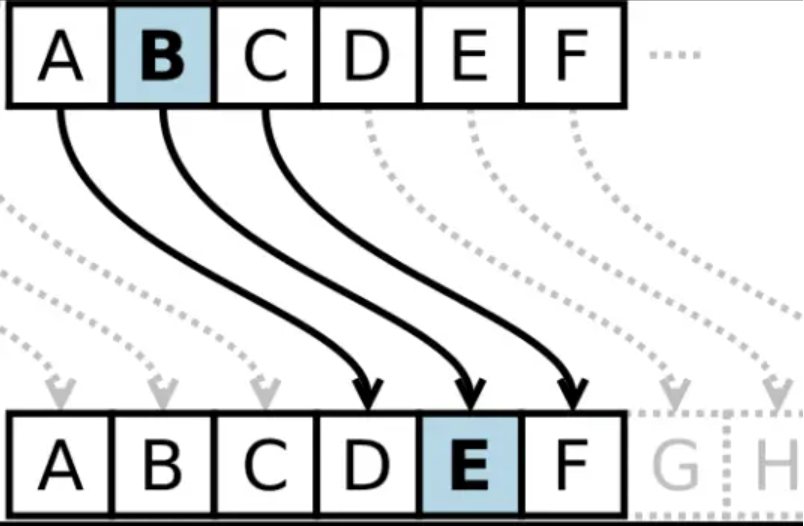
\includegraphics[width=0.5\textwidth]{assets/figures/image-20250210174403824.png} %插入图片,[]中设置图片大小,{}中是图片文件名
    \caption{恺撒加密示意图} %最终文档中希望显示的图片标题
    \label{fig:caesar} %用于文内引用的标签
}

那么现在我们同样用GPT来实现一个这样简单的例子:

\prompt{现在我想编写一个将自然语言转化为恺撒密码的代码,偏移量为3,使用Python代码实现,就以\texttt{My\ Fault\ forgive\ me\ for\ saying\ I\ like\ you\ here}这个句子为例实现一下。
}


\begin{gptbox}
\footnotesize{好的!凯撒密码是一种替换加密技术,每个字母在字母表上向后移动固定的位数(这里是3位)。例如,`A'会被转换为'D',`B'会变成'E',依此类推。对于字母表的末尾字母(如'X'、`Y'、`Z'),它们会循环回到字母表的开头。

以下是将自然语言转化为凯撒密码的Python代码实现:
}
\small{
以下是统一后的结果:
\begin{lstlisting}[language=Python]
    def caesar_cipher(text, shift=3):
        result = []
        for c in text:
            if c.isupper():
                # 处理大写字母
                new_char = chr((ord(c) - ord('A') + shift) % 26 + ord('A'))
                result.append(new_char)
            elif c.islower():
                # 处理小写字母
                new_char = chr((ord(c) - ord('a') + shift) % 26 + ord('a'))
                result.append(new_char)
            else:
                # 非字母字符保持不变
                result.append(c)
        return ''.join(result)
    # 示例句子
    sentence = "My Fault forgive me for saying I like you here"
    encrypted_sentence = caesar_cipher(sentence, shift=3)
    print("加密后的句子:", encrypted_sentence)
\end{lstlisting}
}
\end{gptbox}

上述代码解释如下:

\begin{enumerate}
  \def\labelenumi{\arabic{enumi}.}

  \item
        \texttt{caesar\_cipher}函数接受两个参数:\texttt{text}(要加密的文本)和\texttt{shift}(偏移量,默认为3)。
  \item
        遍历输入文本中的每个字符。
  \item
        对于大写字母,计算其在字母表中的新位置,并将结果转换回字符。
  \item
        对于小写字母,同样进行处理。
  \item
        非字母字符(如空格、标点符号等)保持不变。
  \item
        将所有处理后的字符拼接成最终的加密字符串。
\end{enumerate}

最后,通过本地运行代码可以得到最终加密结果。输入句子:``My Fault forgive me for saying I like you here'',加密后的输出为``Pb Idxow irujlyh ph iru vdblqj L olnh brx khuh'',如\reffig{fig:caesar-example}。

\fig[h]{

\includegraphics[width=0.7\textwidth]{assets/figures/image-20250210173814654.png} %插入图片,[]中设置图片大小,{}中是图片文件名
  \caption{恺撒加密输出图} %最终文档中希望显示的图片标题
  \label{fig:caesar-example} %用于文内引用的标签
}

Eulooldqw!(Brilliant!)现在你可以用恺撒密码对你想说的话进行加密了,你可以尝试继续让GPT改进,让它可以解密恺撒密码,动手试试看吧!